\documentclass[11pt]{article}
\usepackage[preprint]{acl}
\usepackage{times}
\usepackage{latexsym}
\usepackage[T1]{fontenc}
\usepackage[utf8]{inputenc}
\usepackage{microtype}
\usepackage{inconsolata}
\usepackage{booktabs}
\usepackage{graphicx}
\usepackage{amsmath}
\title{Reproducing LLM-A*: Separating Waypoint Guidance\protect\\from Heuristic Weighting}
\author{SWE3011 Independent Reproduction --- Branch \texttt{gm}\\
Experiment date: 13 October 2026}
\begin{document}
\maketitle
\begin{abstract}
We reproduce the 14-condition structure of Table 1 in \citet{meng2025} using 1,000 public path-planning queries, three original prompts, and two accessible OpenAI model snapshots. GPT-4o mini replaces Llama3 to match the course evaluation model; GPT-3.5 Turbo retains a connection to the original model family. We preserve the released search behavior and record 6,000 model responses. GPT-4o mini Few-shot LLM-A* uses 44.85\% of A* operations with 102.65\% relative path length and 100.00\% validity. However, a same-engine, LLM-free $g+2h$ control uses only 34.32\% of A* operations. A validity-gated proposal reduces operations relative to LLM-A*, but does not establish an advantage over that inexpensive control. We report failures, implementation ambiguities, paired uncertainty, and the limits of these findings.
\end{abstract}

\section{Problem and reproduction objective}
LLM-A* combines language-model suggestions with grid search: the model supplies waypoints, while the search constructs a collision-free route. The course assignment requires reproducing the principal comparison, explaining discrepancies and limitations, and implementing an improvement with evidence. Our contribution is an auditable reproduction and a modest validation/fallback extension, not ownership of the original algorithm or a new search-theoretic guarantee.

We use all 100 maps and 10 start--goal pairs per map from the released dataset. The nominal $50\times30$ environment is stored with exclusive upper bounds $[0,51]$ and $[0,31]$, corresponding to outer walls at 50 and 30. Horizontal and vertical obstacles are closed line segments. Search uses the original eight moves with Euclidean edge costs. The final goal remains fixed: suggested waypoints are heuristic targets, not mandatory path constraints.

\section{Method and implementation fidelity}
For goal $G$, active waypoint $T$, and cost-so-far $g$, the released implementation prioritizes
\begin{equation}
 f(n)=g(n)+\|n-G\|_2+\|n-T\|_2.
\end{equation}
It advances the target when a generated neighbor equals $T$, before checking collision or membership in CLOSED. It then rebuilds every OPEN entry. CLOSED is not reopened, duplicate queue pops count as operations, and the storage count includes infinite-cost entries in the $g$ dictionary. These details are preserved, including the strict waypoint boundary filter and the discrepancy between obstacle endpoint filtering and segment collision checks.

Our separate implementation caches collision results and uses a set for CLOSED membership without removing duplicate expansions. We checked 90 search executions on 30 prespecified queries against the untouched upstream code: paths, operation counts, storage counts, and lengths agreed. We also checked 3,000 continuous segments against Shapely and compared the 30 baseline lengths with an independently implemented Dijkstra search. Final auditing verifies all 1,000 A* lengths against Dijkstra, revalidates every successful recorded route, and checks 62 actual model outputs against upstream search. Input mutation is prevented. Unreachable and identical-endpoint inputs return structured results instead of the upstream exceptions; these changes are documented rather than attributed to the paper.

\paragraph{Dynamic weighted A*.}
The paper specifies initial weight 2 and decay 0.99, but the repository lacks this baseline. We decay after each non-goal pop, clamp the weight at 1, and rekey remaining OPEN entries. This is our explicit interpretation. It yields 59.27\% operations, 78.52\% storage and 100.24\% length, versus the paper's 60.91, 78.53 and 100.24. Similar values do not prove identical implementations.

\section{Experimental setup}
Models are \texttt{gpt-4o-mini-2024-07-18} and \texttt{gpt-3.5-turbo-0125}; both returned their requested snapshot IDs. The assignment permits accessible models and primarily evaluates GPT-4o mini. Llama3 is not evaluated here, so this is a reproduction with a disclosed model substitution, not an exact repetition of both original models.

We load the original Few-shot (five examples), CoT (three), and RePE (three) templates unchanged. RePE is a single prompted generation, not an external iterative feedback loop. Each complete template is sent as one user message to Chat Completions, with temperature 0 and a 1,000-token output limit. The released GPT wrapper instead uses the legacy instruct Completion API and a newline stop. We remove that stop to permit multiline reasoning; this is a material API/termination difference. We do not request JSON-constrained output, repair coordinates, or regenerate poor paths.

The 30-query pilot selects pairs 0--2 in maps 0,10,\ldots,90. Its 180 responses are included in the 6,000 total because settings remain unchanged. Each response is shared between LLM-only and LLM-A* evaluation. Transport failures are bounded and recorded separately from poor generations. All 6,000 requests succeeded at the API level; 229 ended at the token limit. A successful HTTP request is not equivalent to a valid generated path. Generations, request settings, response model IDs, token usage, request IDs, timestamps, file hashes and code hashes are retained. No API key is included in the artifact.

\subsection{Metrics and denominators}
For a metric $m$, we compute the percentage
\begin{equation}
100\exp\left(\frac{1}{N}\sum_{i=1}^{N}\log\frac{m_i}{m_i^{A*}}\right).
\end{equation}
Lower is better; 44.59\% usage means a 55.41\% reduction. Operation and storage are code counters, not CPU instruction counts or bytes. A valid route must connect the specified endpoints, stay inside the boundary and avoid every obstacle; search routes must also use the eight legal moves.

LLM-only evaluates the raw parsed polyline without search-based repair. Operation/storage are undefined for this method. The paper does not fully specify treatment of failed paths in length aggregation. We report length conditional on validity with its explicit sample count. Validity always uses all 1,000 queries. A continuous polyline can be shorter than an eight-connected grid optimum, so such values do not imply a superior grid-optimal route. Paired comparisons use common successes and report their sample counts; failed runs remain in reliability statistics. In this run, no query is valid under all six LLM-only conditions, so a six-way common-success length comparison is undefined.

\begin{table*}[t]
\centering\small
\begin{tabular}{lllrrrrr}
\toprule
Method & Model & Prompt & Op.\% & Storage\% & Length\% & Valid\% & Length $N$\\
\midrule
A* & -- & -- & 100.00 & 100.00 & 100.00 & 100.00 & 1000 \\
Dynamic WA* & -- & -- & 59.27 & 78.52 & 100.24 & 100.00 & 1000 \\
LLM-only & M & Few-shot & -- & -- & 116.64 & 5.60 & 56 \\
LLM-only & M & CoT & -- & -- & 122.00 & 6.50 & 65 \\
LLM-only & M & RePE & -- & -- & 117.95 & 7.30 & 73 \\
LLM-only & G & Few-shot & -- & -- & 109.36 & 6.40 & 64 \\
LLM-only & G & CoT & -- & -- & 126.54 & 7.90 & 79 \\
LLM-only & G & RePE & -- & -- & 157.36 & 12.10 & 121 \\
LLM-A* & M & Few-shot & 44.85 & 64.43 & 102.65 & 100.00 & 1000 \\
LLM-A* & M & CoT & 46.78 & 65.63 & 102.58 & 100.00 & 1000 \\
LLM-A* & M & RePE & 50.22 & 68.32 & 102.35 & 100.00 & 1000 \\
LLM-A* & G & Few-shot & 40.41 & 61.34 & 102.26 & 100.00 & 1000 \\
LLM-A* & G & CoT & 55.96 & 74.34 & 102.80 & 100.00 & 1000 \\
LLM-A* & G & RePE & 72.49 & 86.55 & 102.39 & 100.00 & 1000 \\
\bottomrule
\end{tabular}
\caption{Measured reproduction of the Table 1 structure; every row has 1,000 attempted queries. M=GPT-4o mini snapshot 2024-07-18; G=GPT-3.5 Turbo 0125. Missing metrics are undefined, not zero. Length uses valid paths only; original paper values are separately transcribed in Appendix~\ref{app:paper}.}
\label{tab:reproduction}
\end{table*}

\section{Results and discrepancy analysis}
Table~\ref{tab:reproduction} is generated from saved case-level records. Across both models and three prompts, LLM-A* uses between 40.41\% and 72.49\% of A* operations. GPT-3.5 Few-shot yields 40.41\% operations, 61.34\% storage and 102.26\% length. The paper's GPT-3.5 Few-shot hybrid values are 57.39\% operations, 74.96\% storage, 102.44\% length and 100\% validity. Our differences can reflect snapshot/API changes, output termination, parser behavior and undocumented experimental details. We do not identify one cause without a controlled experiment.

The strict two-coordinate parser flags 32 schema-invalid responses and 382 responses without a matching list. LLM-only validity ranges from 5.60\% to 12.10\%. In contrast, hybrid search validity is 100\% in this dataset even when its model output is not a valid route. A missing coordinate list falls back to start/goal in the released code, making $T=G$ and therefore $f=g+2h_G$. This is different from ordinary A*. Unevaluable list expressions can cause upstream failures. Conversely, triples are silently interpreted using their first two values, even when the model has echoed an obstacle list. We preserve that behavior in the hybrid reproduction and separately flag the schema violation; LLM-only and V-Gate require genuine two-coordinate points. This distinction matters when interpreting the paper's reported 100\% validity.

\subsection{Does the LLM explain the reduction?}
We compare against the same search engine with $T$ fixed at $G$, requiring no LLM call. It achieves 34.32\% operations, 56.23\% storage and 102.02\% length, with 100\% validity. All six hybrid conditions have larger aggregate operation ratios than this no-LLM control. This does not imply the control wins on every individual query. Thus the reduction relative to A* alone does not isolate the contribution of language-model waypoints. A useful claim requires a stronger weighted-search control. This observation applies to the tested implementation and data, not every possible LLM-guided planner.

\section{Proposed method: validity-gated guidance}
The pilot exposed collision-prone polylines and coordinate-schema violations. We propose V-Gate: accept the original LLM-A* guidance only when the complete suggested polyline has correct endpoints, stays in bounds, avoids obstacles, and uses integer coordinates. Otherwise use the same-engine $g+2h_G$ fallback. The rule is fixed for every map and does not use observed per-map performance. It introduces no new model requests or result-dependent retries.

\begin{enumerate}
\item Generate once using the selected original prompt and parse coordinates.
\item Validate the full polyline and integer target coordinates.
\item If accepted, run the original LLM-A* search; otherwise run target=goal search.
\item Validate and report the returned route and all counters.
\end{enumerate}

This gate is a hypothesis about guidance reliability, not a guarantee of better guidance: feasible polylines may still be long, while collision-prone polylines can contain useful soft hints. We test it rather than assuming success. The gate also prevents malformed model output from crashing the proposed planner. No optimality or universal completeness theorem is claimed.

\begin{table}[t]
\centering\small
\setlength{\tabcolsep}{3pt}
\begin{tabular}{lrrrr}
\toprule
Method (M, Few-shot) & Op.\% & Store\% & Len.\% & Valid\%\\
\midrule
A* & 100.00 & 100.00 & 100.00 & 100.00 \\
LLM-A* & 44.85 & 64.43 & 102.65 & 100.00 \\
V-Gate & 34.63 & 56.31 & 102.13 & 100.00 \\
Schema-only & 44.88 & 64.45 & 102.65 & 100.00 \\
A* fallback & 93.25 & 96.87 & 100.19 & 100.00 \\
g+2h & 34.32 & 56.23 & 102.02 & 100.00 \\
\bottomrule
\end{tabular}
\caption{Proposal and ablations on 1,000 queries. Schema-only removes spatial validation but retains a strict two-coordinate schema check; A* fallback replaces the weighted fallback.}
\label{tab:ablation}
\end{table}

For GPT-4o mini Few-shot, V-Gate accepts 56 of 1,000 responses, uses 34.63\% operations and 56.31\% storage, and produces 102.13\% relative length with 100.00\% validity. We resample maps with replacement (2,000 bootstrap replicates, seed 20261013), keeping their within-map pairs together. These intervals describe variation across this map sample; they are not uncertainty over repeated model generations. The paired V-Gate/LLM-A* operation ratio is 77.22\%, with a map-bootstrap 95\% interval [73.98, 80.43]\% over 1000 common-success cases. The no-LLM control is crucial: an improvement over LLM-A* can arise primarily by rejecting its guidance. V-Gate still pays for a model response before rejecting it and should not be advertised as cheaper than LLM-free search.

\begin{figure*}[t]
\centering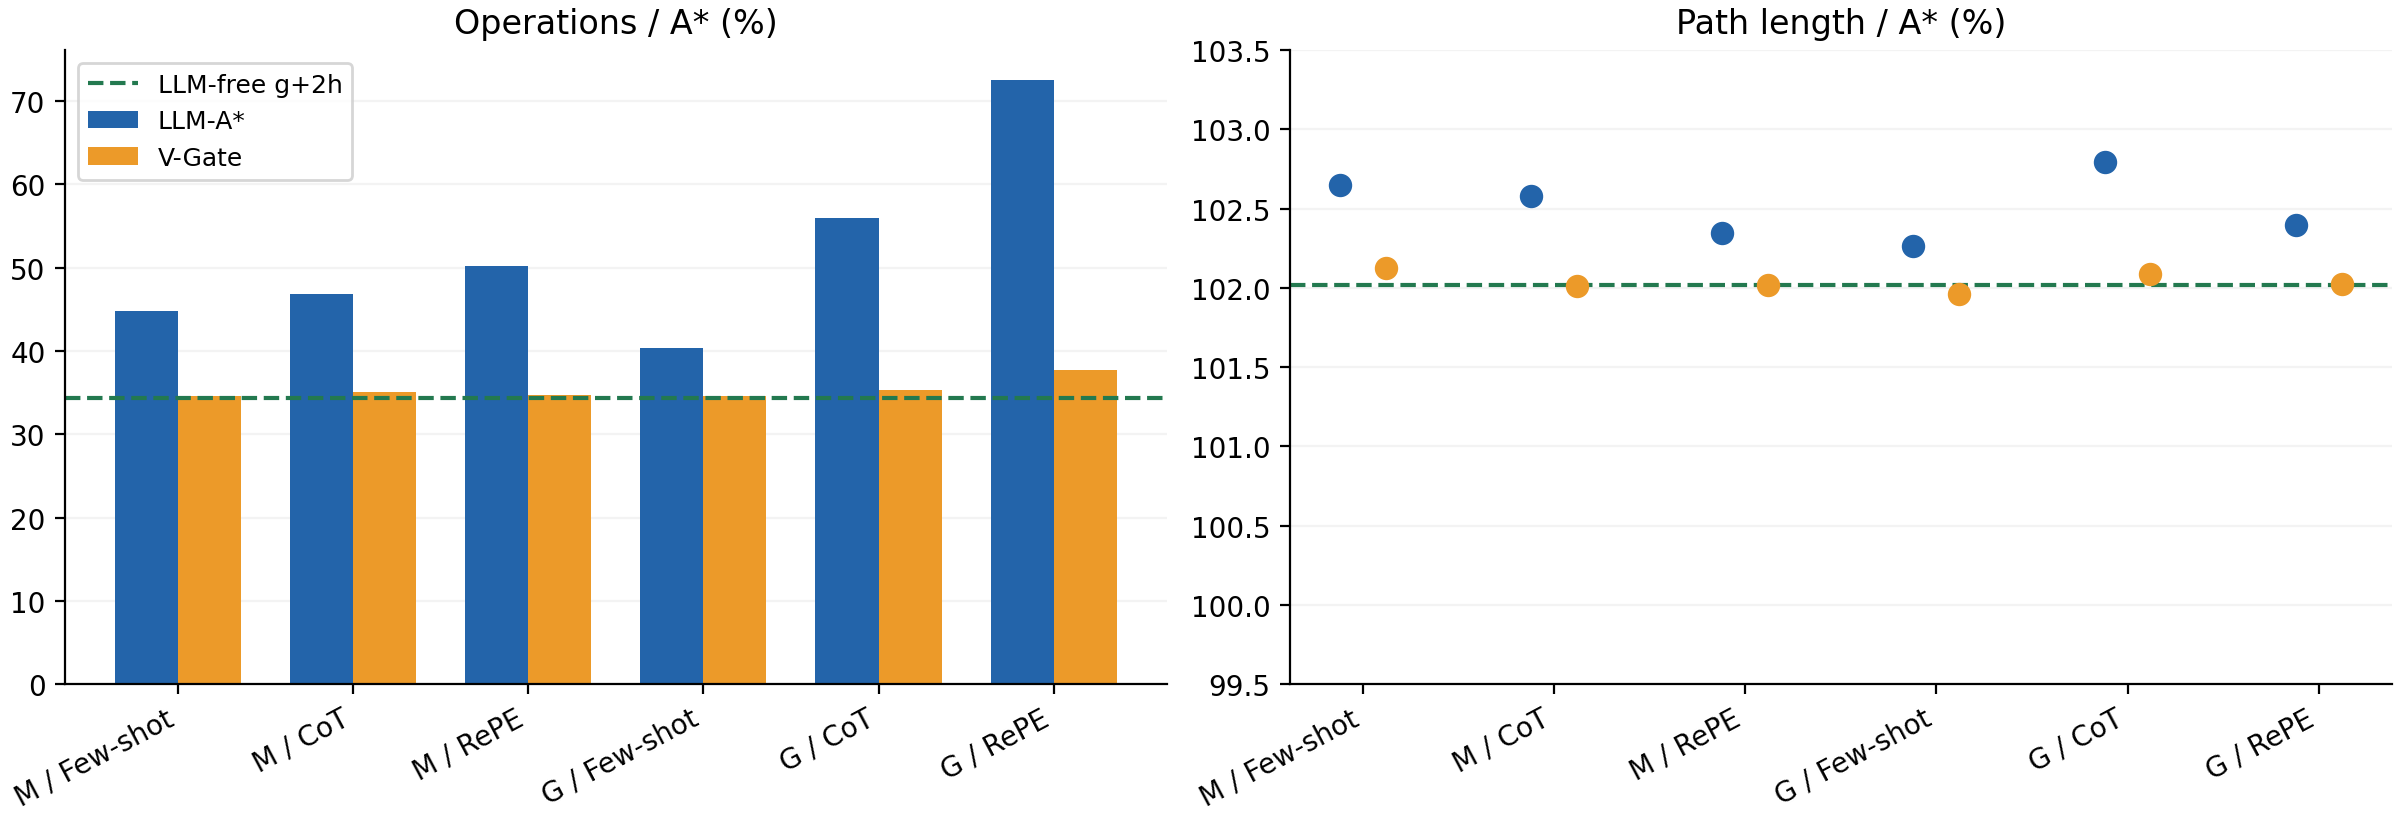
\includegraphics[width=\textwidth]{figures/comparison.png}
\caption{Operation and length ratios for both models and all prompts. The dashed line is the LLM-free $g+2h$ control. Conditional length/operation sample sizes are in the machine-readable tables.}
\end{figure*}

\section{New maps, costs and case analysis}
We generate ten new maps with seed 20261013, four horizontal and four vertical barriers, and three reachable pairs per map. Sizes alternate among $32\times22$, $52\times32$, and $72\times42$. Reachability and baseline length are checked using Dijkstra. The same input adapter and Few-shot template run without map-specific edits; GPT-4o mini produces 30 new responses. LLM-A* and V-Gate both succeed on 30/30 queries. Their operation ratios are 42.12\% and 33.39\%, respectively; the LLM-free control uses 30.51\%. LLM-only succeeds on 9/30. This small smoke evaluation checks portability, not broad generalization. Original prompts omit explicit boundary dimensions, a limitation for varying map sizes.

The main experiment consumed 4,730,480 input tokens and 2,031,098 output tokens, with an estimated standard API cost of USD 3.104. Mean per-request latencies were GPT-3.5 1.81 seconds, GPT-4o mini 4.85 seconds. Estimates use the published standard per-token rates at the time of writing \citep{openai_mini,openai_gpt35}; they are not account invoices. Development access probes and the natural-language adapter smoke test are recorded separately and excluded from the principal 6,000-response usage total. Latency includes service/network delay; cached search replay excludes it. CPU timing in this implementation is not a benchmark of the unmodified plotting-heavy upstream program.

Exact prompt-example overlaps were Few-shot: 5, CoT: 3, RePE: 3. We retain the full dataset for the primary table and supply separate overlap-excluded aggregates; these are not held-out data. Figure~\ref{fig:cases} uses deterministic selections among GPT-4o mini Few-shot joint successes: median and maximum operation ratio relative to $g+2h$, with case ID as tie-breaker. These are illustrative cases, not substitutes for the full distribution. Original LLM outputs, targets and actual paths are saved so a waypoint need not be mistaken for a mandatory visited vertex.

\begin{figure*}[t]
\centering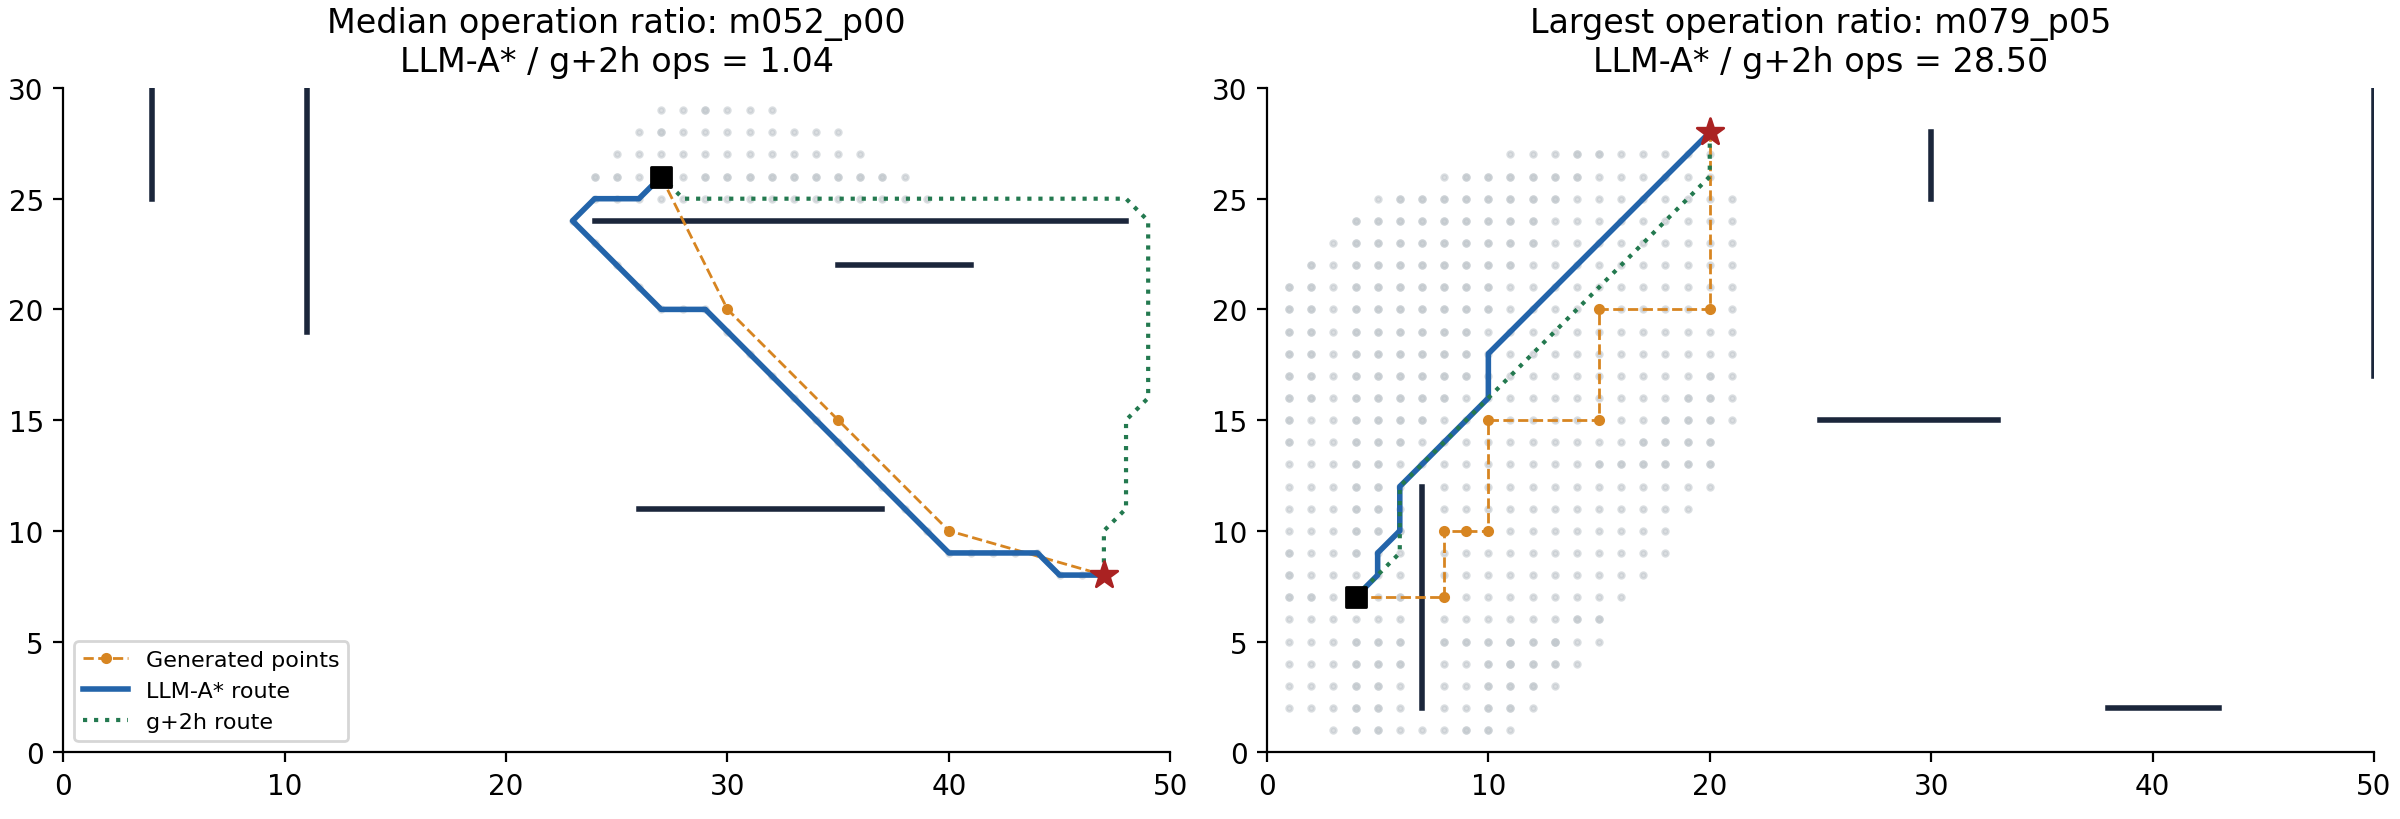
\includegraphics[width=\textwidth]{figures/cases.png}
\caption{Selected original LLM-A* routes (blue), generated waypoint polylines (orange, dashed), and LLM-free control routes (green). Gray points are popped grid states. Case IDs permit replay from the saved records.}
\label{fig:cases}
\end{figure*}

\section{Limitations and reproducibility}
We use one generation per model/prompt/query; temperature zero does not establish deterministic outputs across repeated service calls. The second original model, Llama3, is absent. The DWA interpretation, endpoint geometry, legacy parser, 1,000-token limit and conditional length denominator all limit numerical comparability. The proposal was motivated using a public-data pilot and is not an independently tuned, held-out benchmark result. The new-map set is small. We have not run the paper's ten-scale scalability experiment, which is separate from the assignment's Table 1 target.

The code package provides \texttt{requirements.txt}, a step-by-step README, unchanged upstream sources, generation/evaluation commands, cached responses and per-case records. Models are configurable at runtime for the TA. Structured and natural-language inputs are supported; the latter adds a parsing model call and is not mixed into the Table 1 experiment. Source provenance and implementation differences are documented in \texttt{reproduction/AUDIT.md}. Users can replay search and regenerate tables without credentials.

\section{AI assistance and submission status}
Codex assisted with implementation, checks, experiment orchestration and this draft. Numerical claims come from stored experiments; assistance is not evidence that the student's independent understanding or contribution has been assessed. The student must review the explanation and factual attribution before team submission. This is the independent \texttt{gm} reproduction draft; team authorship/consolidation and individual contribution reports are separate. Individual reports must remain private as required by the assignment. No peer evaluation or response has yet been performed.

\begin{thebibliography}{3}
\bibitem[Meng et al.(2025)]{meng2025} Silin Meng, Yiwei Wang, Cheng-Fu Yang, Nanyun Peng, and Kai-Wei Chang. 2025. \emph{LLM-A*: Large Language Model Enhanced Incremental Heuristic Search on Path Planning}. arXiv:2407.02511v2. Code: \url{https://github.com/SilinMeng0510/llm-astar}, commit \texttt{9414ed8}.
\bibitem[OpenAI(2026a)]{openai_mini} OpenAI. 2026a. GPT-4o mini model documentation. \url{https://developers.openai.com/api/docs/models/gpt-4o-mini}. Accessed 13 October 2026.
\bibitem[OpenAI(2026b)]{openai_gpt35} OpenAI. 2026b. GPT-3.5 Turbo model documentation. \url{https://developers.openai.com/api/docs/models/gpt-3.5-turbo}. Accessed 13 October 2026.
\end{thebibliography}

\appendix
\section{Original reference values}\label{app:paper}
\begin{table*}[t]
\centering\small
\begin{tabular}{lllrrrr}
\toprule
Method & Original model & Prompt & Op.\% & Storage\% & Length\% & Valid\%\\
\midrule
A* & - & - & 100.00 & 100.00 & 100.00 & 100.00 \\
Dynamic WA* & - & - & 60.91 & 78.53 & 100.24 & 100.00 \\
LLM-only & GPT-3.5 & Few-shot & -- & -- & 119.38 & 12.80 \\
LLM-only & GPT-3.5 & CoT & -- & -- & 151.73 & 15.20 \\
LLM-only & GPT-3.5 & RePE & -- & -- & 183.87 & 7.80 \\
LLM-only & Llama3 & Few-shot & -- & -- & 111.05 & 12.60 \\
LLM-only & Llama3 & CoT & -- & -- & 114.89 & 12.00 \\
LLM-only & Llama3 & RePE & -- & -- & 138.32 & 16.40 \\
LLM-A* & GPT-3.5 & Few-shot & 57.39 & 74.96 & 102.44 & 100.00 \\
LLM-A* & GPT-3.5 & CoT & 69.50 & 83.65 & 102.54 & 100.00 \\
LLM-A* & GPT-3.5 & RePE & 85.47 & 96.53 & 102.41 & 100.00 \\
LLM-A* & Llama3 & Few-shot & 44.59 & 64.02 & 102.47 & 100.00 \\
LLM-A* & Llama3 & CoT & 47.60 & 66.27 & 102.46 & 100.00 \\
LLM-A* & Llama3 & RePE & 64.08 & 80.19 & 102.54 & 100.00 \\
\bottomrule
\end{tabular}
\caption{Reference values transcribed from Table 1 of \citet{meng2025}, not measurements from our run. GPT-4o mini has no corresponding original-paper row. Original LLM-only length-denominator details are not fully specified.}
\end{table*}
\end{document}
